%% 
%% Copyright 2016 Icm Ltd
\documentclass[final,3p]{CSP}
\usepackage{amssymb}
\usepackage{changepage}
\begin{document}

\begin{frontmatter}

\title{THESIS PROJECT PROPOSAL}

\author[]{Ashish Sehrawat$^a$}
\author[]{Dr. Jose Feliciano Benitez Rubio$^b$}

%\author[mysecondaryaddress]{Global Customer Service\corref{mycorrespondingauthor}}
%\cortext[mycorrespondingauthor]{Corresponding author}
%\ead{support@Icm.com}

\address[mymainaddress]{Universidad de Sonora}
%\address[mysecondaryaddress]{Universidad de Sonora}

\begin{keyword}\rm
\begin{adjustwidth}{2cm}{2cm}{\itshape\textbf{Keyword:}}  
Higgs boson, Higgs boson production, Higgs boson decay, Higgs boson coupling, 
\end{adjustwidth}
\end{keyword}


\begin{keyword}\rm
\begin{adjustwidth}{2cm}{2cm}{\itshape\textbf{Title:}}  
Study of the Higgs boson production in association with a single top quark in proton collisions at the Large Hadron Collider.
\end{adjustwidth}
\end{keyword}

\begin{abstract}\rm
% \begin{adjustwidth}{2cm}{2cm}{
\itshape\textbf{Abstract:}
The abstract
%\end{adjustwidth}
\end{abstract}


\end{frontmatter}

\section{BACKGROUND}

-SM, Higgs, couplings, previous Higgs measurements, previous tH searches\\

\onehalfspacing The standard model (SM) of particle physics is so far the best theoretical model to describe the interaction of elementary 
particles using three of the four fundamental forces of nature which are electromagnetic force, strong nuclear force and the 
weak nuclear force. Gravitational force is neglected as the strength of this force is very weak at the scales over which 
elementary particle interact with each other. The standard model (SM) of particle physics is divided into two categories, 
bosonic sector and fermionic sector. Bosonic sector contain particles called bosons which mediate the fundamental forces of 
nature and the fermionic sector contain particles called fermions which make up all the matter in our universe. SM has three 
generations of matter (fermions) particles. The first generation of fermions consists of up (u) quark, down (d) quark, electron 
and electron neutrino, second generation consist of charm (c) quark, strange (s) quark, muon and muon neutrino and the third 
generation of matter particles has top (t) quark, bottom (b) quark, tau and tau neutrino. The bosonic sector consist of gauge 
bosons like gluon, photon, $W^{\pm}$, $Z^0$ which mediate strong force, electromagnetic force and weak force respectively. There is one more particle in the standard model called the Higgs Boson which gives mass to SM particles via electroweak symmetry breaking mechanism \cite{Chatrchyan:2012xdj}. Higgs boson can be produced at the particle colliders like the Large Hadron Collider (LHC) in Geneva, Switzerland.\\ 

\begin{figure}
  \centering
   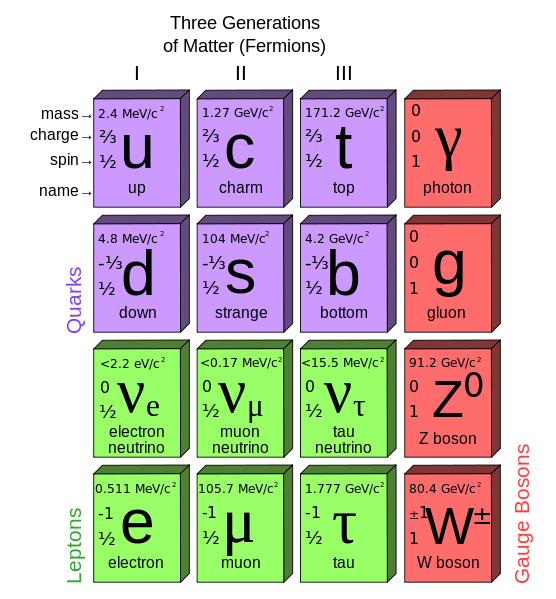
\includegraphics[scale=0.5]{/home/ashish/Desktop/cd11.png}
  \caption{Elementary particles in standard model of particle physics with their mass, spin and charge.}
   \label{figure 1}
\end{figure}

\begin{figure}
  \centering
   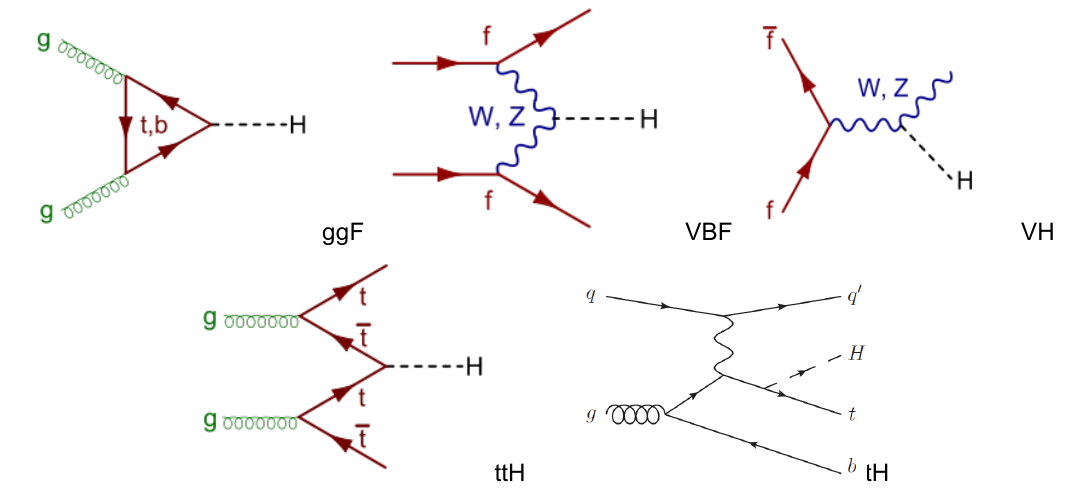
\includegraphics[scale=0.5]{/home/ashish/Desktop/thesis/pg.png}
  \caption{Important production processes of Standard model Higgs boson in proton collisions.}
   \label{figure 2}
\end{figure}

\begin{figure}
  \centering
   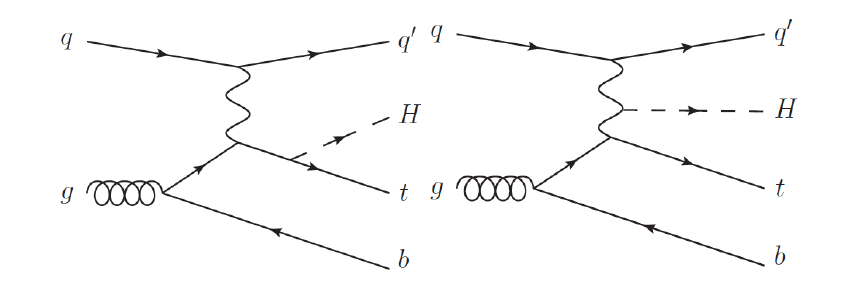
\includegraphics[scale=0.5]{/home/ashish/Desktop/thesis/tq.png}
  \caption{Important production processes of the Higgs boson in proton collisions.}
   \label{figure 3}
\end{figure}

\begin{figure}
  \centering
   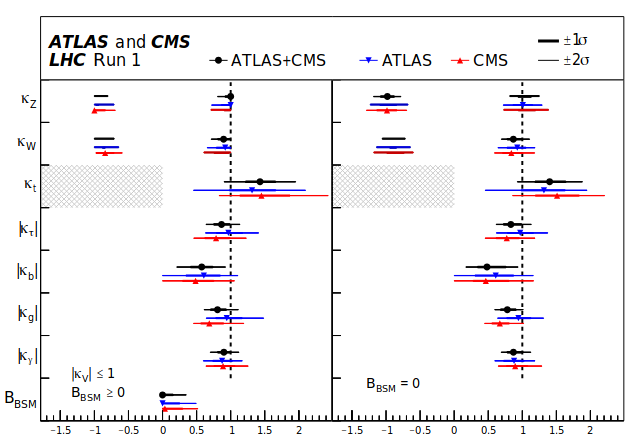
\includegraphics[scale=0.5]{/home/ashish/Desktop/cd7.png}
  \caption{ATLAS-CMS combined measurements of coupling strength modifiers.}
   \label{figure 4}
\end{figure}

\begin{figure}
  \centering
  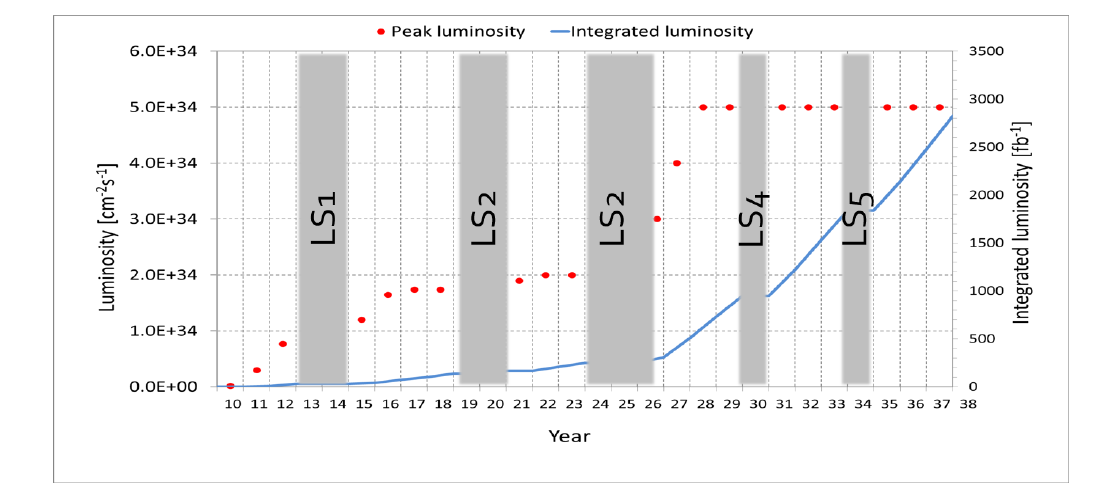
\includegraphics[scale=0.5]{/home/ashish/Desktop/thesis/lum6.png}
  \caption{\onehalfspacing Projected performance of the LHC until 2038, which shows the dates
Preliminary for prolonged stops (LS) of the LHC and luminosities. Points
show instant brightness while the line shows brightness accumulated.}
   \label{figure 5}
\end{figure}

\begin{figure}
  \centering
  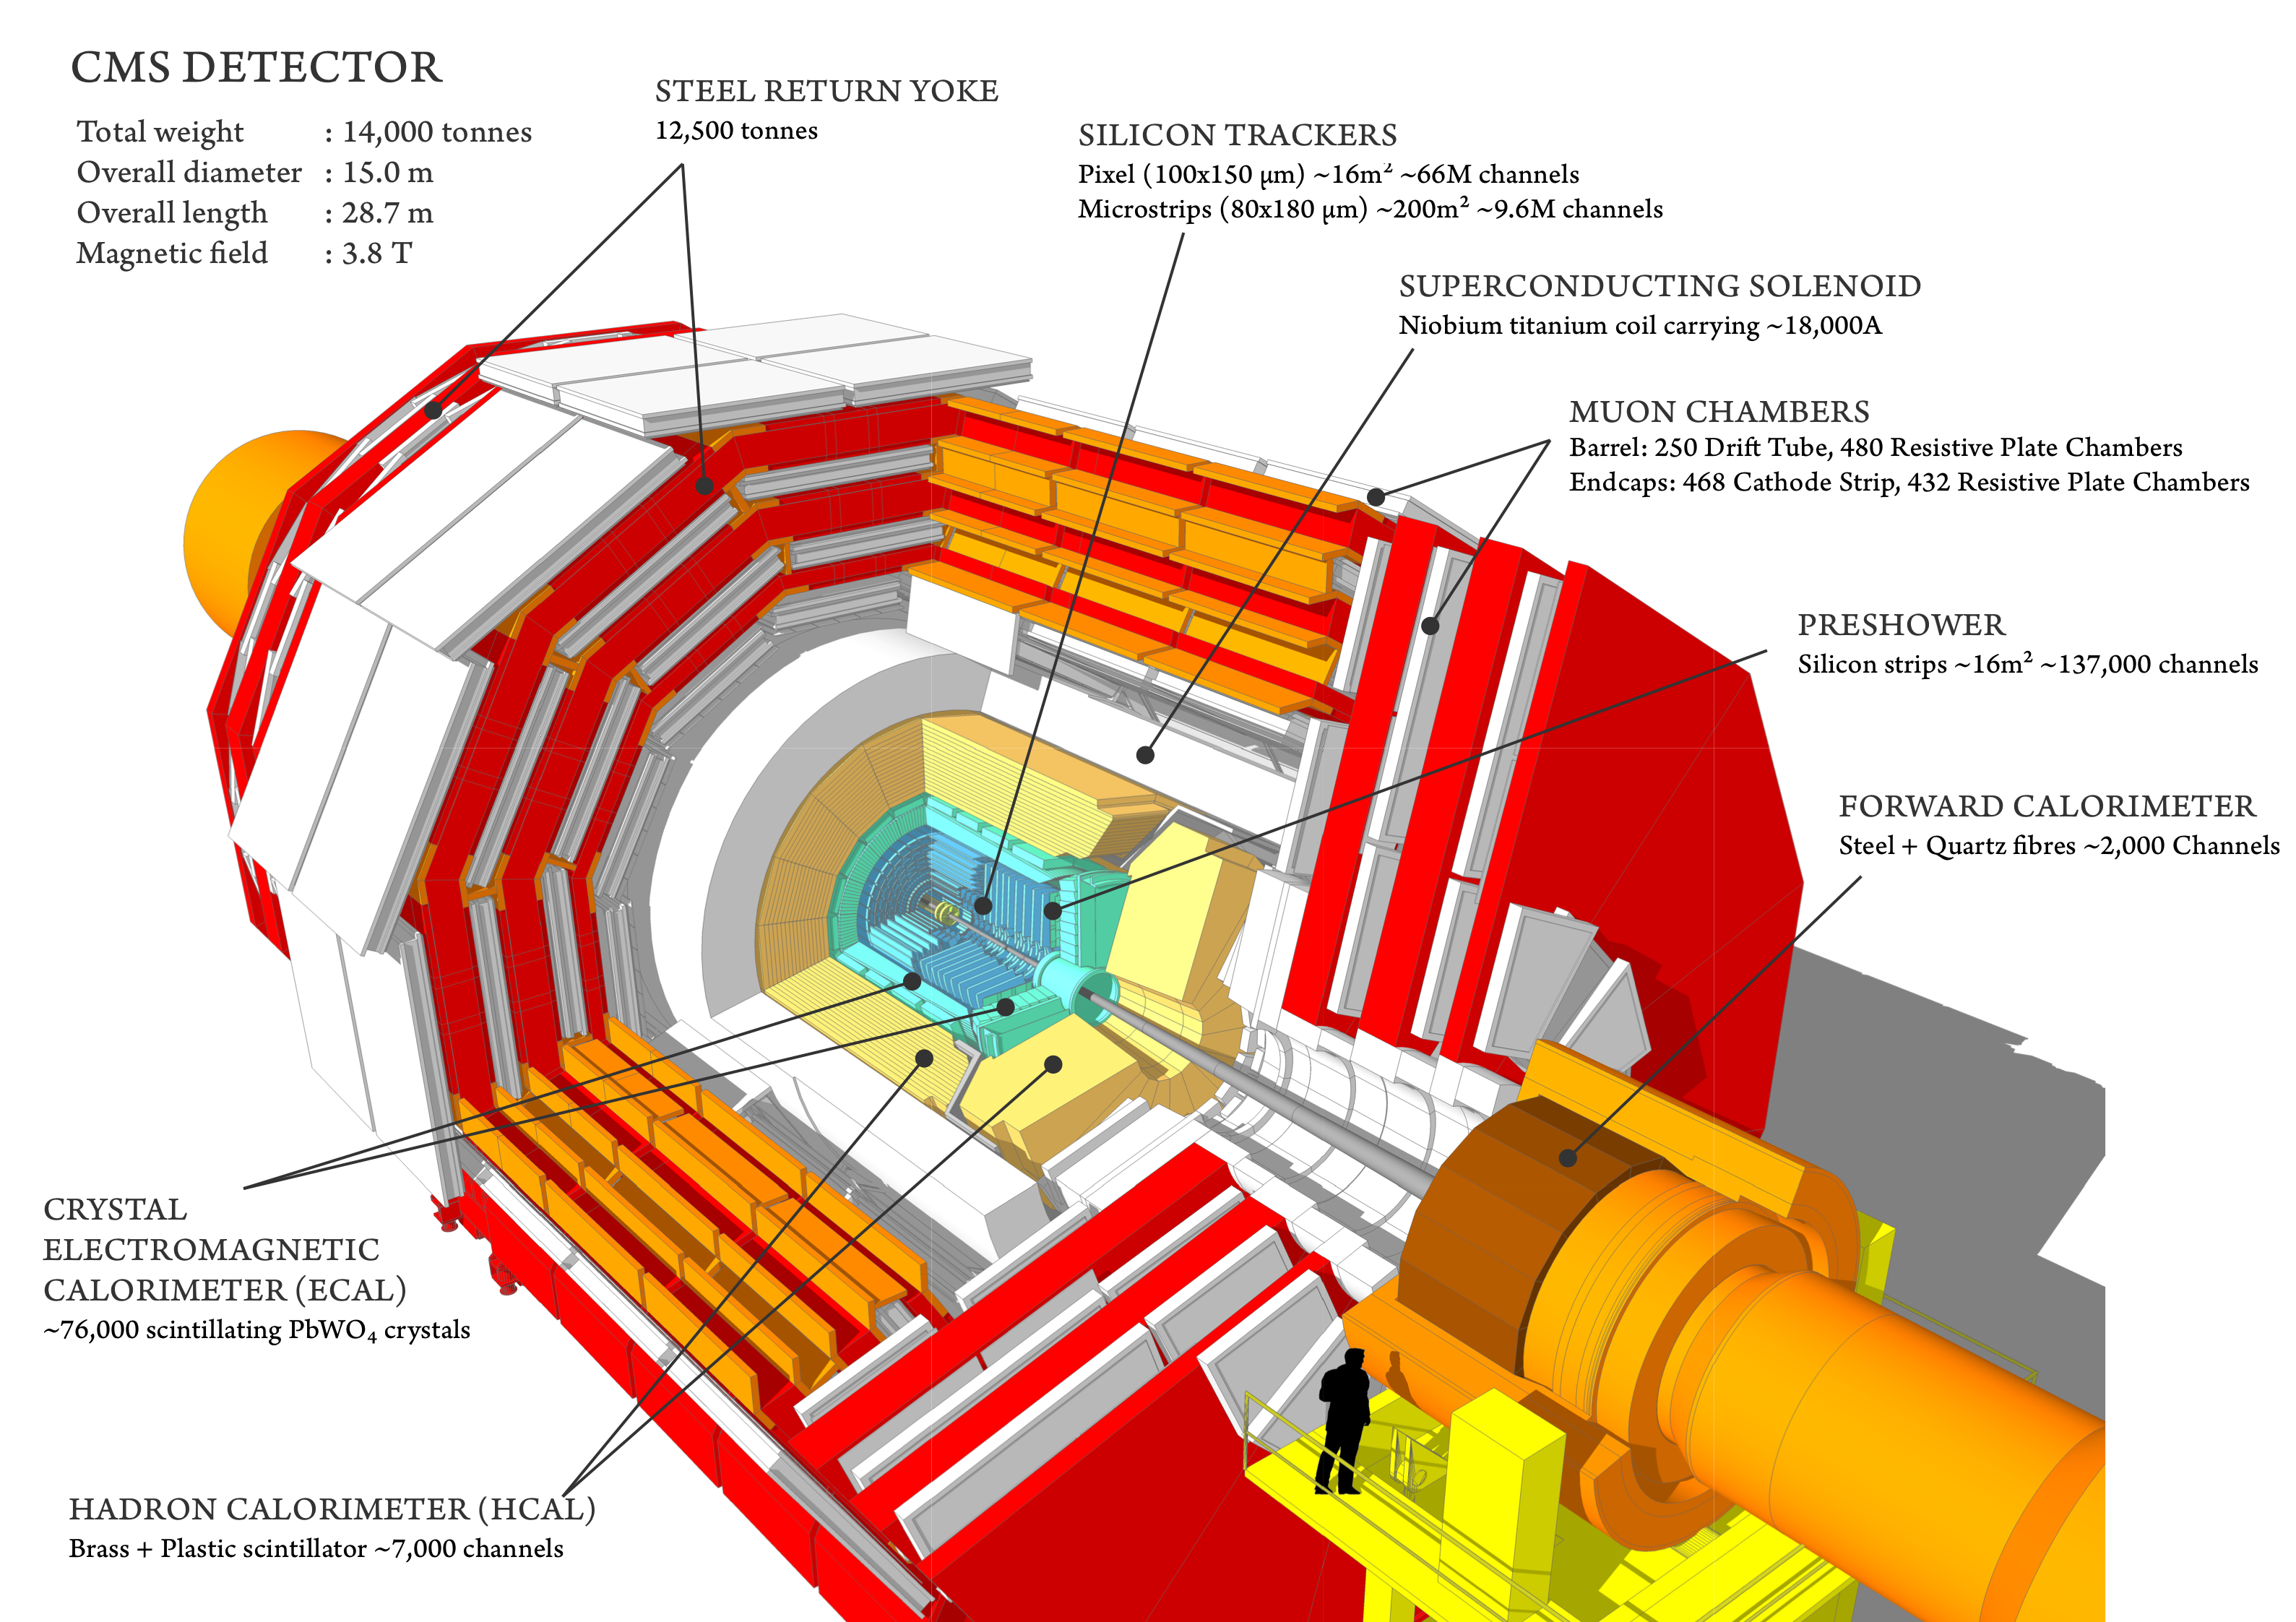
\includegraphics[width=\columnwidth]{/home/ashish/Desktop/thesis/cms.png}
  \caption{\onehalfspacing Leading order Feynman diagrams for the associated production of a single top quark and a Higgs boson in the t channel, where the Higgs boson couples either to the top quark (left) or the W boson (right).}
   \label{figure 6}
\end{figure}

\begin{figure}
  \centering
  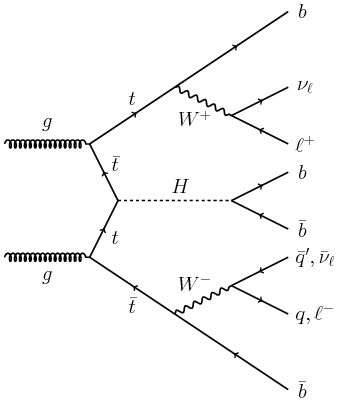
\includegraphics[scale=0.5]{/home/ashish/Desktop/thesis/cms5.png}
  \caption{\onehalfspacing Standard model Higgs boson production in association with top quark and top anti-quark, top quarks decaying to W boson and bottom quark, W boson decaying to leptons.}
   \label{figure 7}
\end{figure}


Until the 90's the existence of almost all the particles of the SM were confirmed except the top quark and the Higgs boson. 
These had eluded previous experiments due to difficulties in the production or reconstruction of its decays. The top quark was 
discovered in 1995 in the Tevatron collider of the Fermilab laboratory, this proton collider operated with a center of mass 
energy of 1.8 TeV untill 2010. The LHC collider at the CERN laboratory in Geneva, Switzerland, began its operations in 2010 
colliding protons at 7 TeV increasing the colliding energies to 8 and 13 TeV in the subsequent years. The Compact Muon Solenoid (CMS) is based on the Large Hadron Collider (LHC) located at CERN. It is designed to detect particles known as muons very accurately. The CMS detector has the form of a cylindrical onion, with several concentric layers of components. Needed a powerful magnet to bend charged particles as they move away from the point of collision to identify the charge of the particles to bend them in opposite directions and measure your momentum. A silicon tracker, made of about 75 
million electronic sensors individual arranged in concentric layers, identifies the routes taken by these charged particles bent with very high precision. The muons are not detected by electromagnetic or hadron calorimeters, so special sub-detectors are outside to detect them once they have crossed the solenoid. In 2012, the ATLAS and CMS collaborations, with detectors at two points where the protons collide in the LHC, announced the discovery of a new boson with a mass of 125 GeV. So far, all measurements of the properties of this boson are consistent with those of the Higgs boson of the standard model (SM).\\

There are various production modes of Higgs boson like the gluon gluon fusion (ggF), vector boson fusion (VBF), Higgs 
production in association with vector boson (VH, V = W or Z), Higgs production with top quark and top anti-quark (t$\bar{t}$H) and Higgs 
production with a single top quark and a quark jet (tHq). Each production channel has its own importance to probe the 
properties and the coupling strength of Higgs boson to fermions and bosons. The main production mode of Higgs bosons at LHC is 
gluon gluon fusion (ggF). As bosons like gluons and photons are massless, they do not interact directly with the Higgs boson 
and processes like ggF or Higgs boson decay to pair of photons are not possible at tree level and can only proceed via loop 
diagrams which involve W boson or top quark in the loop. The Higgs boson can also decay to other particles and these decay 
channels have different branching fractions. Higgs boson can decay to a pair of W bosons, Z bosons, photons, bottom quarks, 
muons and electrons. Higgs boson can also decay to Z boson and a photon. It is also interesting to investigate some invisible 
decay modes of Higgs boson which can be used to put upper bounds on dark matter-nucleon scattering cross section like in the 
Higgs-portal dark matter models. \\

The Standard Model (SM) of particle physics has successfully described most of the experimental data till now but a very large 
number of free-parameters like fine structure constant $\alpha$, Weinberg angle or weak mixing angle $\theta_W$, the coupling 
constant of strong interaction, electroweak symmetry breaking energy scale, Higgs potential self coupling or the Higgs mass, 
three mixing angles and the CP-violating phase of the CKM matrix which tells us how quarks of 
different color charge mix with 
each other, nine yukawa couplings which determine the mass of nine charged fermions and fine 
tunings related to the origin of 
masses robustly suggests new physics beyond Standard model (BSM). There are lot of specific 
BSM theories and most of these 
models involve heavy fields. In order to identify which new physics lies beyond the 
electroweak (EW) scale, the new parameters 
of such theories may be constrained by the actual, low energy, experiments. This approach 
requires studying each model 
individually, and calculating every possible observable. There is another approach immitating 
Fermi's treatment of beta decay 
which consists of considering the SM as the first order approximation of the actual theory 
and by completing it with a series 
of higher dimensional operators. When the electroweak symmetry breaking takes place well 
below the mass of the new particles, 
the BSM physics is taken into account at the EW scale and below by adding higher dimensional 
operators to the SM Lagrangian. 
They are built out of SM fields and supposed to be invariant under its gauge group. Those 
operators are the low-energy residue 
of the high energy theory. This approach does not pretend to guess the complete high-energy 
model and it is based solely on 
the symmetry of the  theory. The operators are general and the only model dependence is 
encoded in the size of the operator 
coefficients, which is to be set from experiments. \\

The Higgs boson and fermions (quarks and leptons) coupling will deviate from the standard 
model predictions if these higher 
dimensional operators are present in low energy effective SM theory. We can consider 
anomalous Higgs and Higgs-gauge effective 
dimension 6 operators like $-\frac{1}{3}(\phi^{\dagger}\phi)^3$, $\frac{1}{2} \partial_{\mu} 
(\phi^{\dagger} \phi) 
\partial^{\mu}(\phi^{\dagger} \phi)$ and $(\phi^{\dagger} \phi)(D_{\mu} \phi)^{\dagger} 
(D^{\mu} \phi)$ to calculate the 
deviation of Higgs boson-fermion couplings from SM. The first operator shift the minimum of 
the Higgs potential. Also as there 
will be rescaling of the Higgs field due to the introduction of these operators in the 
potential term, Higgs-fermion (quarks 
and leptons) couplings are modified. In the effective standard model theory, there are 
dimension 5 and dimension 6 
operators. Dimension 5 operators are odd under baryon minus lepton number symmetry and 
dimension 6 operator dominate baryon 
minus lepton number symmetry conservation processes. \\

The production of Higgs boson in association with single top quark is one of the rare Higgs 
boson production mode \cite{Khachatryan_2016}. As the top 
quark is the heaviest fundamental particle in the standard model, due to its large mass, the 
top quark decay before 
hardronization which allow the possibility to reconstruct top quark from its decay products 
unlike the lighter quarks which 
undergo hardronization and are seen as bundles of particles in detector called jets. The most 
probable decay of top quark is 
into bottom (b) quark and W boson \cite{nishiwaki2014tth}. Using b-jet tagging algorithms, the jet originating from 
b-quark can be reconstructed to 
identity the top quark. In SM, the coupling of the Higgs boson to fermions like quarks and 
leptons is proportional to the mass 
of the fermions. Thus heavy quarks like top, bottom and charm couple strongly to Higgs boson 
which means that out of all known 
quarks, top quark couple most strongly to the Higgs boson. So, it has a large value of Yukawa 
coupling $y_t$ \cite{Aad_2016}. That is why the 
Yukawa coupling of the top quark with the Higgs boson $y_t$ has lot of importance as any 
deviation from standard model prediction might give an indication of new physics. The two 
processes at LHC which will allow us to directly probe the Yukawa 
coupling between Higgs Boson and top quark are Higgs boson production in association with top 
quark pair (t$\bar{t}$H) via 
strong interaction and the production of single top quark with a Higgs boson (tH). As tH 
occur via electroweak interaction, it 
is more rare than t$\bar{t}$H production \cite{sirunyan2018search}. The Higgs boson in the tH channel can be radiated 
off by a W boson or by a top 
quark. These two processes in standard model have destructive interference which allow us to 
probe the relative sign between 
the coupling of top quark with Higgs boson $y_t$ and the coupling of W boson to the Higgs 
boson \cite{choudhury2019search}. If the Yukawa coupling between top quark and Higgs boson $y_t$ deviate from the SM 
prediction or even if $y_t$ has a negative sign, both would cause a strong increase in the tH 
production cross section which is a special property of tH production channel making it an 
interesting production channel to probe using LHC 2016, 2017 and 2018 data. The coupling 
strength modifier $\kappa_t$ is defined as $\kappa_t = \frac{y_t}{y^{SM}_t}$ which will tell 
us the deviation of $y_t$ from the SM prediction. 
The LHC is sensitive to an anamolous Higgs coupling to the top quark in the Higgs boson-top 
quark associated production mode. 
The anomalous coupling will arise when we add interaction terms (dimension 6 operators in 
effective SM theory) in the Higgs 
potential. As there is strong destructive inteference in the t-channel for the standard model 
couplings, this production mode 
is sensitive to both the sign and the magnitude of any coupling beyond the SM between Higgs 
boson and top quark induced by 
higher dimensional operators in effective SM theory \cite{sirunyan2019search}.

\section{PROPOSAL}

- what we will do:  search for tH events, using which channels.

\onehalfspacing In this project, it is proposed to study the production channel of the Higgs boson associated 
with a single top quark in the Large Hadron Collider of the CERN laboratory. The measurement 
of this process complements other measurements of the yukawa coupling parameter of the top 
quark and Higgs boson. It is a part of the physics program of CMS international 
collaborations and ATLAS and it has not been observed so far. It is proposed to study 
sensitivity with the current data in the channel where the events are identified with two 
muons of the same sign. The impact of uncertainties will be studied and projections will be 
made to the future phases of the LHC. For these studies the data of the run two (2015-2018) 
of the LHC identifying the signal events with two muons from the same sign. It is also 
expected to estimate projections for the high brightness phase of the LHC (HL-LHC) that began 
in 2026. 

\section{GENERAL OBJECTIVE}

- motivation, tH production crossection, sign of $k_t$, search for BSM, ..

\onehalfspacing There is currently a great enigma in physics since we know that ordinary matter comprises 
only $5\%$ of the universe, another 
$27\%$ includes what we call dark matter. Understanding the production of the Higgs boson, as 
well as its decays like the invisible decay modes are an important part of the physics 
program of CERN laboratory experiments to verify the Standard Model and look for new 
particles. Through this project we will investigate the production of the Higgs boson in 
association with a single top quark (tH) in proton-proton collisions with the CMS experiment 
of the LHC. We will study the distribution of events in one of the decay channels and the 
sensitivity that we get with the current data. The main objective is to search for new 
processes such as tH Higgs production mode in the CMS experiment which require to study 
different aspects such as the model of the noises that are made by simulation, techniques of 
adjustments to the data that incorporate the different noises and the signal, and estimates 
of statistical and systematic uncertainties.
Some of the objectives in this project include:\\
\begin{itemize}
\item study one or more decay channels.\\
\item verify that simulation of signal events is adequate.\\
\item study the extraction of signal strength through adjustments to the data.\\
\item study the impact of statistical and systematic uncertainties.\\
\end{itemize}

\section{SPECIFIC OBJECTIVES}
- details 

\section{HYPOTHESIS}
- what we expect to find

\onehalfspacing Production studies in the tH channel have already started with the collaborations CMS and 
ATLAS with publications based on data from the 2011-2012 run and some data from the second 
run of 2015-2016. In these results it was not found signal evidence and upper limits have 
been set for the effective section. With the more sensitive analysis an upper limit is 
calculated for the effective section of a signal composed of tH and ttH that corresponds 3.1 
times that expected in the SM. In this analysis the reconstruction methods do not allow to 
distinguish between tH and t$\bar{t}$H because the effective section of t$\bar{t}$H is much 
larger than that of tH and some events pass the selections designed for tH, the fraction of 
tH events over tH + t$\bar{t}$H is 5. In BSM models the fraction could change up to 50, for 
example with $\kappa_t = -1$. It could help to obtain better limits for the production of tH. 
The data that has been used so far correspond to only 20 of the final data of the run that 
which ends in 2018. The uncertainty for the signal in the current analysis is mostly 
statistical nature, therefore adding the total data in a new analysis the next year, 
sensitivity can be improved with an approximate factor of 2.2. Additionally, in subsequent 
phases of the LHC 2021-2023 and 2026-2038 the number of data fold and then multiply by 10 
respectively. With these additions It is expected that the signal from the Higgs boson can be 
observed on the tH production channel. The current results can be used to project sensitivity 
in the third run and the high brightness phase and thus contribute to the planning of the 
updates of the detector.

\section{METHODOLOGY}
- methods used in the search: which dataset,  lepton reconstruction, selections, jets, BDT, backgrounds, statistical analysis

\onehalfspacing Aspects of simulation of signal production are studied based on generators that simulate the 
interactions of quarks and gluons taking into account the probability distributions of each 
type of particle. These are packages of software that are controlled with configuration files 
that define various aspects of such as decay channels, energy in the center of mass and 
refinements in the development of the jets that are generated by the strong interaction of 
the quarks. The reconstruction and selection of tH events requires the use of central 
software of the CMS collaboration. This software contains the algorithms that reconstruct the 
charged and neutral particles starting from the energy deposits in the different parts of the 
detector. These particles include leptons, photons and hadrons which have a life time that 
allows them to leave the interaction region. These particles are used to identify the 
production of the top and the Higgs boson. In the case of the top quark, it usually decays to 
a bottom (b) quark and a W boson. Subsequently the W decays to two leptons or two quarks. 
Reconstruction requires finding a type b and two jet leptons. Improvements in this 
reconstruction can be done by studying the distributions of transverse momentum, the angular 
distributions of the different particles, and others properties.

\section{EXPECTED RESULTS}
- a limit, also predictions for future runs

The expected results of this project are the following:
• Improve data adjustments and study the effects of uncertainties.
• Improve the sensitivity to the tH signal in the data of the second CMS run.
• Limit calculations in the effective section incorporating data from the second
run of the LHC.
• Calculate projections of signal sensitivity for the different phases of the LHC.

\bibliographystyle{unsrt}
\cleardoublepage
\bibliography{paper}


\appendix
\section{SKILLS THAT WILL BE DEVELOPED}
The following are skills that will be developed based on the work on this project:
- understand particle physics from an experimental point of view.
- analyze and manipulate data using modern programming languages such as C++, Python and ROOT.
- data analysis techniques.
- use high performance computing.

\section{CALENDAR OF ACTIVITIES}

\newpage
\cleanpage


\begin{figure}
  \centering
   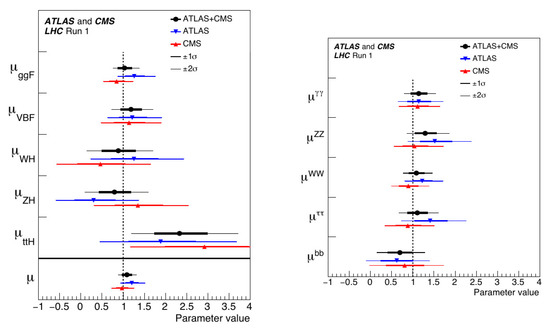
\includegraphics[width=\columnwidth]{/home/ashish/Desktop/thesis/cms7.jpg}
  \caption{Higgs boson signal strength modifier in various production modes and decay channels.}
   \label{figure 10}
\end{figure}

\begin{figure}
  \centering
   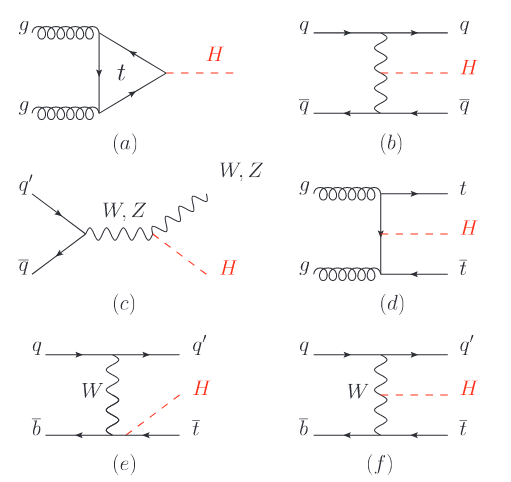
\includegraphics[width=\columnwidth]{/home/ashish/Desktop/cd.png}
  \caption{Leading order Feynman Diagrams for various Higgs production modes.}
   \label{figure 12}
\end{figure}


\begin{figure}
  \centering
   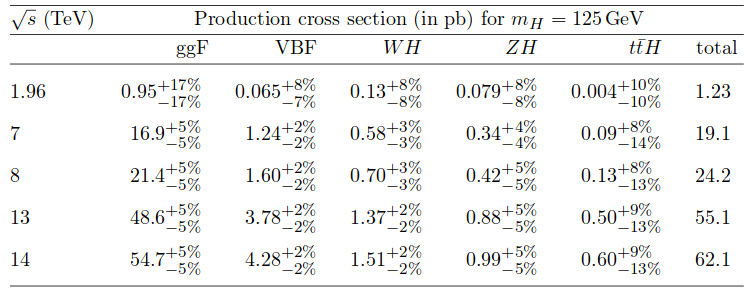
\includegraphics[width=\columnwidth]{/home/ashish/Desktop/cd1.png}
  \caption{Standard model Higgs boson production cross section in various production modes.}
   \label{figure 13}
\end{figure}

\begin{figure}
  \centering
   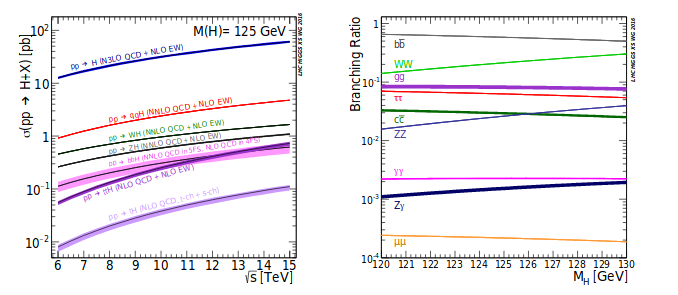
\includegraphics[width=\columnwidth]{/home/ashish/Desktop/cd2.png}
  \caption{Standard model Higgs boson production cross section with center of mass energy and branching ratios for various decay channels.}
   \label{figure 14}
\end{figure}

\begin{figure}
  \centering
   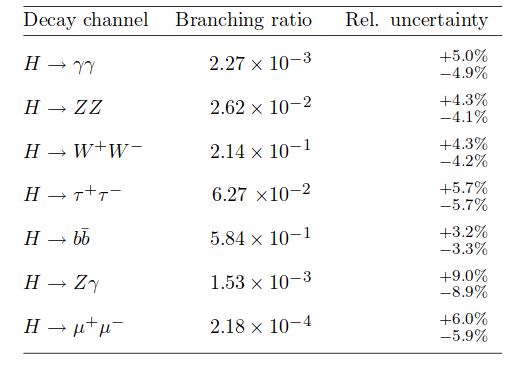
\includegraphics[width=\columnwidth]{/home/ashish/Desktop/cd3.png}
  \caption{Standard model Higgs boson branching ratios in various decay channels.}
   \label{figure 15}
\end{figure}


\begin{figure}
  \centering
   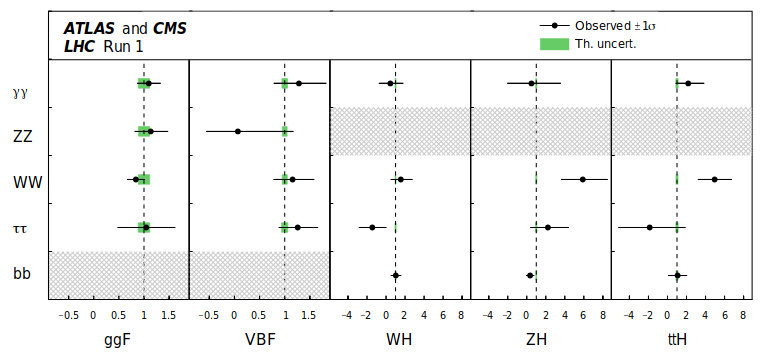
\includegraphics[width=\columnwidth]{/home/ashish/Desktop/cd5.png}
  \caption{Combined measurement of the products $\sigma$.BR for various production and decay channels of Standard model Higgs boson.}
   \label{figure 17}
\end{figure}

\begin{figure}
  \centering
   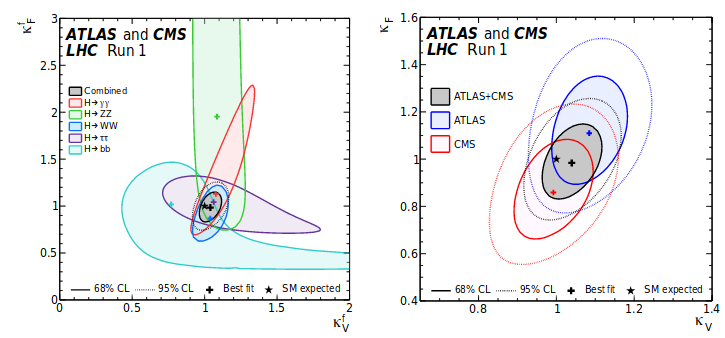
\includegraphics[width=\columnwidth]{/home/ashish/Desktop/cd6.png}
  \caption{Likelihood contours in the ($\kappa_F$,$\kappa_V$) plane and combined fit for all decay channels.}
   \label{figure 18}
\end{figure}


\begin{figure}
  \centering
   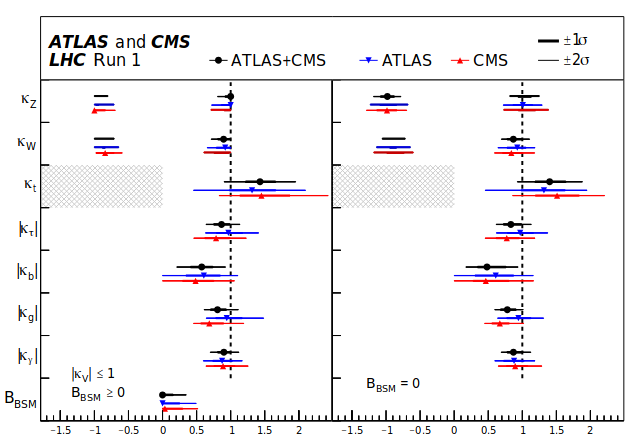
\includegraphics[width=\columnwidth]{/home/ashish/Desktop/cd7.png}
  \caption{ATLAS-CMS combined measurements of coupling modifiers.}
   \label{figure 19}
\end{figure}

\begin{figure}
  \centering
   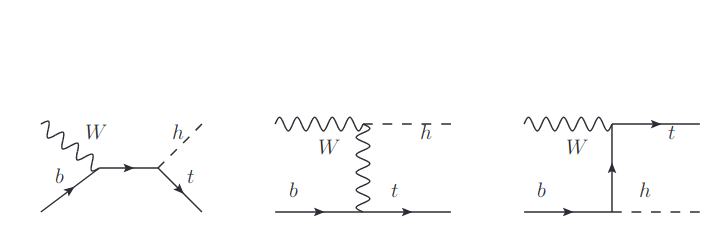
\includegraphics[width=\columnwidth]{/home/ashish/Desktop/th.png}
  \caption{Feynman diagrams contributing to the partonic process W b $->$ tH.}
   \label{figure 20}
\end{figure}

\begin{figure}
  \centering
   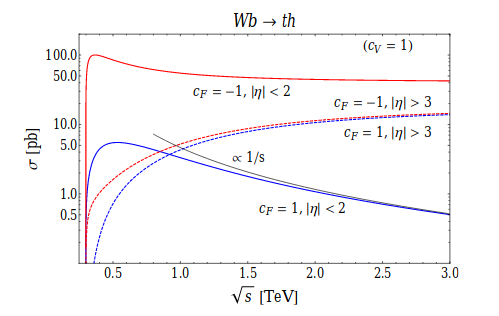
\includegraphics[width=\columnwidth]{/home/ashish/Desktop/th1.png}
  \caption{Partonic cross sections for the process W b $->$ tH as a function of the center of mass
energy.}
   \label{figure 21}
\end{figure}

\begin{figure}
  \centering
   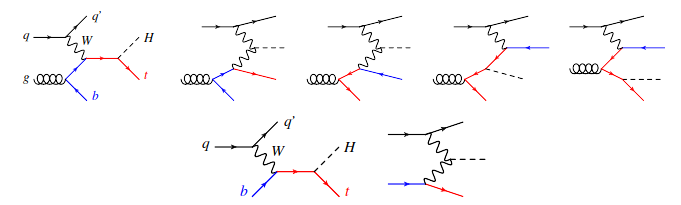
\includegraphics[width=\columnwidth]{/home/ashish/Desktop/th2.png}
  \caption{Lowest order Feynman diagrams for t-channel tH production in the 4F scheme and in the 5F scheme.}
   \label{figure 22}
\end{figure}

\begin{figure}
  \centering
   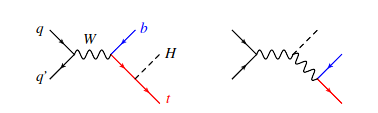
\includegraphics[width=\columnwidth]{/home/ashish/Desktop/th3.png}
  \caption{Lowest order Feynman diagrams for s-channel tH production.}
   \label{figure 22}
\end{figure}


\end{document}


